\documentclass[border=15pt]{standalone}
\usepackage{tikz}
\usetikzlibrary{arrows.meta, positioning, calc}
\usepackage{amsmath}

\begin{document}

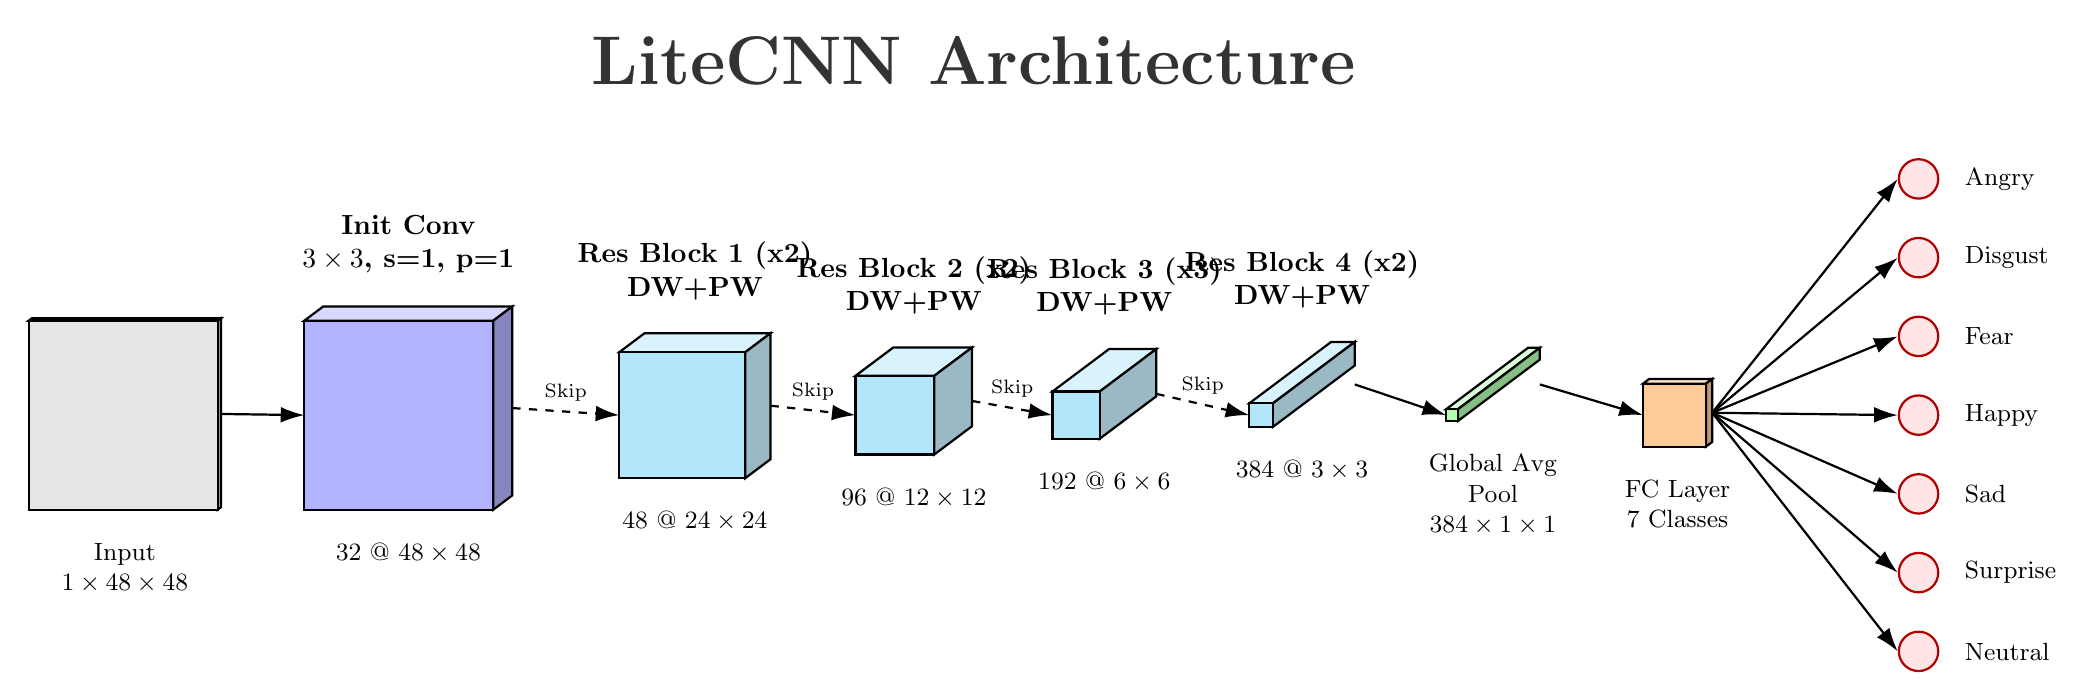
\begin{tikzpicture}[
    x=1cm, y=1cm,
    font=\sffamily,
    >= {Latex[length=3mm, width=2mm]},
    ]

    % Define a macro to draw each 3D layer block
    \newcommand{\networklayer}[7]{
        \def\posx{#2}
        \def\spat{#3}
        \def\chan{#4}

        % Perspective projection adjustments
        \pgfmathsetmacro{\cx}{\chan * 0.4}
        \pgfmathsetmacro{\cy}{\chan * 0.3}

        % 【安全颜色解析】
        \colorlet{basecolor}{#5}
        \colorlet{frontcolor}{basecolor}
        \colorlet{topcolor}{basecolor!50!white}
        \colorlet{sidecolor}{basecolor!75!black}

        % Draw Top Face
        \draw[fill=topcolor, thick] (\posx, \spat/2) -- (\posx + \spat, \spat/2) -- (\posx + \spat + \cx, \spat/2 + \cy) -- (\posx + \cx, \spat/2 + \cy) -- cycle;
        % Draw Right Face
        \draw[fill=sidecolor, thick] (\posx + \spat, -\spat/2) -- (\posx + \spat + \cx, -\spat/2 + \cy) -- (\posx + \spat + \cx, \spat/2 + \cy) -- (\posx + \spat, \spat/2) -- cycle;
        % Draw Front Face
        \draw[fill=frontcolor, thick] (\posx, -\spat/2) rectangle (\posx + \spat, \spat/2);

        % Define Anchor Coordinates for arrows
        \coordinate (in-#1) at (\posx, 0);
        \coordinate (out-#1) at (\posx + \spat + \cx, \cy/2);
        
        % Label Nodes
        \node[align=center, anchor=south, yshift=0.3cm, font=\bfseries] at (\posx + \spat/2 + \cx/2, \spat/2 + \cy) {#6};
        \node[align=center, anchor=north, yshift=-0.3cm, font=\small] at (\posx + \spat/2 + \cx/2, -\spat/2) {#7};
    }

    % ==========================================
    % Draw Network Layers (LiteCNN Architecture)
    % Parameters: ID, X_pos, Spatial_Scale, Channel_Scale, Color, Top_Label, Bottom_Label
    % ==========================================

    % 1. Input
    \networklayer{input}{0}{2.4}{0.1}{gray!20}{}{Input \\ $1 \times 48 \times 48$}

    % 2. Init Conv (Different color to distinguish from ResBlocks)
    \networklayer{init}{3.5}{2.4}{0.6}{blue!30}{Init Conv \\ $3\times3$, s=1, p=1}{32 @ $48 \times 48$}

    % 3. Res Block 1
    \networklayer{res1}{7.5}{1.6}{0.8}{cyan!30}{Res Block 1 (x2) \\ DW+PW}{48 @ $24 \times 24$}

    % 4. Res Block 2
    \networklayer{res2}{10.5}{1.0}{1.2}{cyan!30}{Res Block 2 (x2) \\ DW+PW}{96 @ $12 \times 12$}

    % 5. Res Block 3
    \networklayer{res3}{13.0}{0.6}{1.8}{cyan!30}{Res Block 3 (x3) \\ DW+PW}{192 @ $6 \times 6$}

    % 6. Res Block 4
    \networklayer{res4}{15.5}{0.3}{2.6}{cyan!30}{Res Block 4 (x2) \\ DW+PW}{384 @ $3 \times 3$}

    % 7. Global Avg Pool
    \networklayer{gap}{18.0}{0.15}{2.6}{green!30}{}{Global Avg \\ Pool \\ $384 \times 1 \times 1$}

    % 8. FC Layer
    \networklayer{fc}{20.5}{0.8}{0.2}{orange!40}{}{FC Layer \\ 7 Classes}

    % ==========================================
    % Draw Arrows Between Layers
    % ==========================================
    \draw[->, thick] (out-input) -- (in-init);
    \draw[->, thick, dashed] (out-init) -- (in-res1) node[midway, above, font=\scriptsize] {Skip};
    \draw[->, thick, dashed] (out-res1) -- (in-res2) node[midway, above, font=\scriptsize] {Skip};
    \draw[->, thick, dashed] (out-res2) -- (in-res3) node[midway, above, font=\scriptsize] {Skip};
    \draw[->, thick, dashed] (out-res3) -- (in-res4) node[midway, above, font=\scriptsize] {Skip};
    \draw[->, thick] (out-res4) -- (in-gap);
    \draw[->, thick] (out-gap) -- (in-fc);

    % ==========================================
    % Draw Output Nodes (7 Emotion Classes)
    % ==========================================
    \coordinate (node_start) at (24.0, 0);

    \foreach \name/\y/\label in {
        angry/3/Angry, 
        disgust/2/Disgust, 
        fear/1/Fear, 
        happy/0/Happy, 
        sad/-1/Sad, 
        surprise/-2/Surprise, 
        neutral/-3/Neutral} 
    {
        % Draw circular nodes
        \node[circle, draw=red!70!black, fill=red!10, thick, minimum size=0.5cm] (outnode-\name) at (24.0, \y) {};
        
        % Draw class text
        \node[right=0.2cm of outnode-\name, font=\small] {\label};
        
        % Draw arrows from FC to nodes
        \draw[->, thick] (out-fc) -- (outnode-\name.west);
    }

    % ==========================================
    % Title
    % ==========================================
    \node[font=\Huge\bfseries, align=center, text=black!80] at (12, 4.5) {LiteCNN Architecture};

\end{tikzpicture}

\end{document}
